%==============================================================================
% Over-the-Air Normalized Aggregation with Private Weights -- IEEE TWC submission.
% IEEEtran, double-column journal style. Build: latexmk -pdf main.tex (aux files go to build/).
% Tables in tables/ are generated by pwna/p8_tables.py; every number in the text is in
% results/p8_analysis/summary.md or paper_numbers.md (results/p8, results/p7, results/p8_supp).
%==============================================================================
\documentclass[journal]{IEEEtran}
\usepackage{amsmath,amssymb,amsthm,amsfonts}
\usepackage{graphicx,booktabs,array,multirow}
\graphicspath{{figures/}}
\usepackage{algorithm,algpseudocode}
\usepackage{xcolor}
\usepackage[hidelinks]{hyperref}

\theoremstyle{plain}
\newtheorem{theorem}{Theorem}
\newtheorem{lemma}{Lemma}
\newtheorem{corollary}{Corollary}
\newtheorem{proposition}{Proposition}
\theoremstyle{definition}
\newtheorem{definition}{Definition}
\theoremstyle{remark}
\newtheorem{remark}{Remark}

\newcommand{\R}{\mathbb{R}}
\newcommand{\C}{\mathbb{C}}
\newcommand{\E}{\mathbb{E}}
\newcommand{\Prob}{\mathbb{P}}
\newcommand{\vh}{\mathbf{h}}
\newcommand{\vm}{\mathbf{m}}
\newcommand{\vn}{\mathbf{n}}
\newcommand{\vo}{\mathbf{o}}
\newcommand{\vz}{\mathbf{z}}
\newcommand{\vq}{\mathbf{q}}
\newcommand{\vk}{\mathbf{k}}
\newcommand{\vv}{\mathbf{v}}
\newcommand{\obar}{\bar{\mathbf{o}}}
\newcommand{\Neff}{N_{\mathrm{eff}}}
\newcommand{\snr}{\mathrm{SNR}}
\makeatletter\newcommand{\tabinput}[1]{\@@input #1 }\makeatother  % expandable \input for generated table bodies
\newcommand{\FXBITS}{37}   % ring size of the secure aggregation, eps = 1e-6 (results/p7/p7_f5_fx_*.json, max over models)

\setlength{\textfloatsep}{6pt plus 2pt minus 2pt}
\setlength{\floatsep}{6pt plus 2pt minus 2pt}
\setlength{\intextsep}{6pt plus 2pt minus 2pt}
\setlength{\dbltextfloatsep}{6pt plus 2pt minus 2pt}

\begin{document}

\title{Over-the-Air Normalized Aggregation with Private Weights: Extreme-Value Analysis and Split-Ratio Design for Distributed Attention}

\author{Mengqi Hu%
\thanks{The author is with the Ming Hsieh Department of Electrical and Computer Engineering, University of Southern California, Los Angeles, CA, USA (e-mail: mengqihu@usc.edu).}}

\markboth{IEEE TRANSACTIONS ON WIRELESS COMMUNICATIONS, SUBMITTED 2026}{HU: OVER-THE-AIR NORMALIZED AGGREGATION WITH PRIVATE WEIGHTS}

\maketitle

\begin{abstract}
Normalized aggregation $\sum_j d_j\obar_j/\sum_j d_j$ with weights computed locally from a query---the softmax merge of context-parallel attention, kernel regression---maps onto over-the-air computation as the ratio of two superposed sums. With private weights, the common scale is set by the mass-weighted weakest link. We show that this bottleneck obeys an exact Fr\'echet law with scale $\sum_j d_j^2/\beta_j$, derive the outage and saturation laws, and prove a converse: a scale that never saturates and reveals $k$ bits per instance loses at least $W2^{-k-1}$~dB on a range of $W$~dB. Going beyond it requires saturation, which we make harmless and controlled. Devices securely aggregate the weights with which they actually arrive, so the ratio stays a convex combination, and they announce a noise-matched level that bounds every device's distortion by $\kappa$ noise variances and makes the bottleneck bounded. The fusion center learns one quantized maximum and one sum. In sharded-KV decoding of three LLMs with up to 128 devices and 32k-token contexts, the design is near-lossless at $-8$ to $8$~dB, 5--12~dB below a non-saturating split ratio and within 0.2--4.1~dB of the strongest known-weight baseline, and it is up to 14 times faster than a secure digital merge of matched accuracy. It also outperforms adaptively weighted averaging on spatial-field regression.
\end{abstract}

\begin{IEEEkeywords}
Over-the-air computation, normalized aggregation, extreme-value analysis, power control, distributed attention, large language models, secure aggregation.
\end{IEEEkeywords}

%==============================================================================
\section{Introduction}
\label{sec:intro}
%==============================================================================

\IEEEPARstart{L}{arge} language models (LLMs) are increasingly asked to reason over contexts that do not fit in, or must not leave, a single machine: long documents, multi-party logs, or private records held by different edge devices. Context-parallel decoding addresses this by sharding the key--value (KV) cache along the sequence dimension: every shard computes a partial attention for the current query and the partial results are merged by a log-sum-exp (LSE) reduction~\cite{lin2024infinite,acharya2025star,bhatia2025helix,shyam2024tree}. The merge message of a shard is a single vector and a single scalar~\cite{acharya2025star}, and the merge itself is a \emph{normalized aggregation}
\begin{equation}
\vo=\frac{\sum_{j}\vn_j}{\sum_{j}d_j}=\frac{\sum_j d_j\obar_j}{\sum_j d_j},\qquad d_j=\sum_{i\in\mathcal{S}_j}e^{s_i-c},
\label{eq:intro_merge}
\end{equation}
where $s_i$ are the attention logits of the tokens in shard $\mathcal{S}_j$, $c$ is a common shift and $\obar_j$ is the shard's local attention output. The same structure appears in kernel (Nadaraya--Watson) regression of spatial fields, where $d_j$ is a kernel of the distance between the query location and sensor~$j$, and in product-of-experts Gaussian-process regression, where $d_j$ is the local posterior precision~\cite{sato2022gpr,sato2026awa}.

Because both the numerator and the denominator of~\eqref{eq:intro_merge} are sums, over-the-air computation (AirComp)~\cite{nazer2007computation,goldenbaum2015nomographic,sahin2023survey} can produce them in one shot by letting all devices transmit simultaneously, after which the fusion center (FC) divides. For attention, one aggregation instance per layer and head occupies $d_v+1$ real channel uses regardless of the number of devices~$N$. The difficulty is that the weights are \emph{private}: $d_j$ is computed at device~$j$ from the broadcast query and its own data, it is unknown to the FC, it is heavy-tailed, and it changes with every query. Weight-aware AirComp designs~\cite{cao2020power,liu2020scaling,yang2026airmoe,zhang2026logit} assume that the transmit weights are known to the server, and the only ratio-type AirComp scheme with locally computed weights~\cite{sato2026awa} collects the message norms digitally before every slot and clips the weights with bounds tuned by Bayesian optimization, without a closed-form analysis. With private weights, the scale that every device must share is limited by the \emph{mass-weighted weakest link} $\max_j d_j^2/g_j$, where $g_j$ is the effective channel gain---a quantity the FC cannot observe.

This paper develops the theory and the designs for this setting and validates them on two applications: sharded-KV LLM decoding and spatial-field estimation.

\textbf{Contributions.}
\begin{itemize}
\item \emph{Model.} We formalize private-weight normalized AirComp under the per-device peak-power convention of~\cite{yang2026airmoe}, with an $M$-antenna FC whose receive combiner depends on the channels only, and an anchor block held by the FC (Section~\ref{sec:model}). The model covers the LSE merge of context-parallel decoding and kernel/product-of-experts regression, and it treats \emph{what the FC learns} as a design dimension.
\item \emph{Extreme-value analysis.} We show that the mass-weighted inversion bottleneck is exactly Fr\'echet with scale $S=\sum_j d_j^2/\beta_j$ under Rayleigh fading and heterogeneous path loss, and give the product law under Nakagami-$m$ fading (Section~\ref{sec:analysis}). For homogeneous links $S=D^2/\Neff$, so the participation ratio $\Neff$ of the weights acts as an SNR multiplier; the law reduces to~\cite[Cor.~2]{liu2020scaling} and~\cite[Lemma~5]{chen2024view} for equal weights. We derive the denominator outage in closed form, the conditions under which the ratio estimator has finite moments, and the saturation law of any weight-blind scalar design, whose \emph{price of blindness} grows with the dispersion of $S$ across queries; on attention weights the best blind scale needs 19--28~dB.
\item \emph{Converse and designs.} An anonymous ladder handshake lets the FC learn only a quantized $\max_j d_j^2/g_j$. We prove that, among all scales that never saturate and reveal at most $k$ bits per instance, the ladder is optimal and loses $W2^{-k-1}$~dB on a range of $W$~dB, which yields a privacy--accuracy trade-off (Section~\ref{sec:design}). Known-weight designs such as~\cite{yang2026airmoe} do better because they let the bottleneck devices saturate, which a ratio with an exact denominator cannot tolerate. We remove this obstacle with two components. In the \emph{saturation-aware split ratio}, the numerator is sent over the air and the devices securely aggregate~\cite{bonawitz2017secagg} the weights with which they actually arrive, so that the ratio remains a convex combination under any saturation. With the \emph{noise-matched level report}, every device announces the smallest noise level at which its own saturation distortion stays below $\kappa$ noise variances; the resulting bottleneck has a closed-form law, is bounded instead of Fr\'echet, and needs no weight at the FC. The FC learns one quantized maximum and one sum per instance.
\item \emph{Validation.} We verify every closed form by Monte Carlo. On sharded-KV decoding of three LLMs with up to 128 devices and 32k-token contexts, the proposed design needs 5--12~dB less SNR than a non-saturating split ratio and 2--9~dB less than known-weight aggregation at the genie scale; it is on par with or better than the threshold design of AirMoE~\cite{yang2026airmoe} and stays within 0.2--4.1~dB of that design strengthened with our saturation-aware denominator. We report paired confidence intervals, a design study of both components, one-round alternatives, channel impairments, task-level retrieval, the ring size that a secure digital merge needs at the same accuracy, and a latency ledger built on it. On distributed regression of a spatial field with up to 1024 sensors, the design outperforms adaptively weighted averaging~\cite{sato2026awa} without tuned clipping or truncation (Sections~\ref{sec:regime} and~\ref{sec:exp}).
\end{itemize}

\textbf{Related work.} Power control for AirComp in fading channels is well understood when the data to be summed are normalized: threshold-based optimal policies and scaling laws~\cite{cao2020power,liu2020scaling}, multi-antenna receivers~\cite{zhu2019mimo,chen2024view}, and imperfect channel state information (CSI)~\cite{evgenidis2024imperfect}. Ratio-type AirComp with an over-the-air denominator was introduced for product-of-experts regression~\cite{sato2022gpr} and adaptively weighted averaging~\cite{sato2026awa}. AirComp has recently been applied to LLM inference: tensor-parallel all-reduce~\cite{zhang2025jstsp}, mixture-of-experts aggregation with optimal threshold power control~\cite{yang2026airmoe}, and logit-aware MIMO transceivers~\cite{zhang2026logit}; in all of them the aggregation weights are computed and known at the server, and none estimates a denominator. The threshold scale of~\cite{yang2026airmoe} is our strongest baseline, and the noise-matched report can be read as its decentralized counterpart for weights that the server must not see. Systems work on context-parallel decoding~\cite{lin2024infinite,acharya2025star,bhatia2025helix,shyam2024tree,meta2025cp} merges digitally and motivates sharding by memory capacity and data placement, as we do. To our knowledge, the LSE merge of attention has not been studied as an over-the-air ratio with private weights.

%==============================================================================
\section{System Model}
\label{sec:model}
%==============================================================================

\subsection{Normalized Aggregation With Private Weights}

An FC and $N$ single-antenna devices cooperate to compute, for each \emph{aggregation instance},
\begin{equation}
\vo=\frac{\vn_A+\sum_{j=1}^N d_j\obar_j}{d_A+\sum_{j=1}^N d_j}\in\R^{d_v},
\label{eq:target}
\end{equation}
where $(d_A,\vn_A)$ is an anchor term held by the FC, $d_j\ge0$ is the weight of device $j$ and $\obar_j$ its local normalized output, with $\|\obar_j\|\le V_{\max}$. The weights are \emph{private}: $d_j$ is computed at device $j$ from information broadcast by the FC and from data that only device $j$ holds, and the FC does not know $\{d_j\}$ before or after the aggregation. We write $D=\sum_j d_j$ for the device mass and
\begin{equation}
\Neff=\frac{\big(\sum_j d_j\big)^2}{\sum_j d_j^2}\in[1,N]
\label{eq:neff}
\end{equation}
for the participation ratio of the weights: $\Neff=N$ when the mass is spread evenly and $\Neff\approx1$ when one device dominates.

\emph{Sharded-KV attention.} Consider decoding with a KV cache whose context is split into $N$ contiguous shards $\mathcal{S}_j$, one per device. For a query $\vq$ of one head in one layer, device $j$ computes the logits $s_i=\vq^{\mathsf T}\vk_i/\sqrt{d_k}$ of its tokens and returns $d_j=\sum_{i\in\mathcal{S}_j}e^{s_i-c}$ and $\vn_j=d_j\obar_j=\sum_{i\in\mathcal{S}_j}e^{s_i-c}\vv_i$. The FC holds an anchor block (the first tokens, which contain the system prompt and the attention sink~\cite{xiao2024streaming}) and the tail from the question on, including the generated tokens, in the spirit of the anchor block of~\cite{acharya2025star}. It sets $c$ to the maximum of its own logits, so no extra round is needed to agree on the shift, and $(d_A,\vn_A)$ collects its own terms. Then~\eqref{eq:target} is exactly the attention output. Since $\obar_j$ is a convex combination of value vectors, $V_{\max}$ can be taken as the largest value norm of the head, calibrated offline. Fig.~\ref{fig:system} sketches the system and the protocol of Section~\ref{sec:design}.

\begin{figure}[t]
\centering
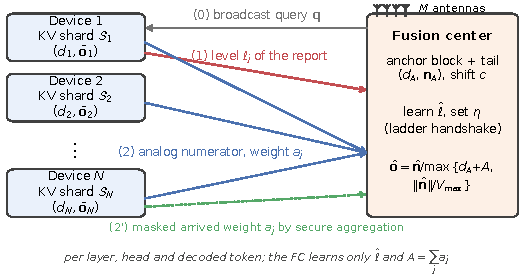
\includegraphics[width=\linewidth]{fig_system.pdf}
\caption{Sharded-KV decoding over the air. Per layer, head and decoded token, the FC broadcasts the query (0); the devices announce the level of their noise-matched report through a digital or tone handshake (1) and transmit their scaled partial outputs, which superpose at the $M$-antenna FC (2); the weights with which they arrive are securely aggregated in parallel (2').}
\label{fig:system}
\end{figure}

\emph{Spatial regression.} In Nadaraya--Watson regression with a Gaussian kernel, $d_j=\exp(-\|\mathbf{x}_\star-\mathbf{x}_j\|^2/2h^2)$ and $\obar_j=y_j$ for a sensor at $\mathbf{x}_j$ with measurement $y_j$ and a query location $\mathbf{x}_\star$; this is softmax attention with distance logits. The FC may add a prior pseudo-observation $(d_A,\vn_A)=(w_0,\mathbf{0})$. In product-of-experts Gaussian-process regression~\cite{sato2022gpr}, $d_j=\sigma_j^{-2}(\mathbf{x}_\star)$ and $\obar_j=\mu_j(\mathbf{x}_\star)$ are the local posterior precision and mean of expert $j$.

\subsection{Channel and Receiver}

The FC has $M$ antennas. The channel of device $j$ is $\vh_j=\sqrt{\beta_j}\,\tilde{\vh}_j\in\C^M$, where $\beta_j$ is the large-scale gain and $\tilde{\vh}_j\sim\mathcal{CN}(\mathbf{0},\mathbf{I}_M)$; the channels are independent across devices and constant over one instance. The FC applies a unit-norm receive combiner $\vm$ chosen from the channels only---it cannot use the weights---and device $j$ sees the effective gain
\begin{equation}
g_j=|\vm^{\mathsf H}\vh_j|^2 .
\end{equation}
For $M=1$, $g_j=\beta_j|\tilde h_j|^2$ is exponential with mean $\beta_j$. In the analysis we also allow Nakagami-$m$ fading, $|\tilde h_j|^2\sim\mathrm{Gamma}(m,1/m)$. Each device knows its effective channel $\vm^{\mathsf H}\vh_j$, which it can estimate from a downlink pilot precoded with $\vm$ under channel reciprocity.

\subsection{Transmission and Estimator}

We adopt the convention of~\cite{yang2026airmoe}: the weight is placed in the precoder and the data are normalized. Device $j$ transmits $d_v+1$ real streams, the denominator stream with datum $1$ and the numerator streams with data $\obar_j/\sigma_o$, where $\sigma_o$ is an offline root-mean-square value of the outputs, all with the same precoder
\begin{equation}
b_j=\frac{\eta\,d_j}{\sqrt{g_j}}\,e^{-\jmath\angle(\vm^{\mathsf H}\vh_j)},\qquad |b_j|^2\le P .
\label{eq:precoder}
\end{equation}
Here $\eta>0$ is a scale common to all devices. A device for which $\eta^2d_j^2/g_j>P$ cannot invert its channel and transmits at full power; its weight then arrives attenuated as $a_j=\sqrt{Pg_j}/\eta<d_j$. In general $a_j=\min\{d_j,\sqrt{Pg_j}/\eta\}$. After combining, phase compensation and normalization by $\eta$, the FC observes
\begin{align}
\hat D&=d_A+\sum_j a_j+\frac{z_0}{\eta}, \label{eq:Dhat}\\
\hat\vn&=\vn_A+\sum_j a_j\obar_j+\frac{\sigma_o}{\eta}\vz, \label{eq:Nhat}
\end{align}
with $z_0\sim\mathcal{N}(0,1)$ and $\vz\sim\mathcal{N}(\mathbf{0},\mathbf{I}_{d_v})$, i.e., real noise of unit variance per stream; the signal-to-noise ratio is $\snr=P$. The FC outputs
\begin{equation}
\hat\vo=\frac{\hat\vn}{\max\{\hat D,\ d_A,\ \|\hat\vn\|/V_{\max}\}},
\label{eq:estimator}
\end{equation}
where the floor is the convex-hull projection of Section~\ref{sec:design}; we call~\eqref{eq:estimator} the \emph{analog ratio}. One instance occupies $d_v+1$ real channel uses whatever $N$ is; an LLM layer with $H$ query heads needs $H(d_v+1)$ real symbols per decoded token.

The design problem is the choice of the scalar $\eta$ for every instance. If the FC knew the weights, the largest scale that avoids saturation would be the \emph{genie} scale
\begin{equation}
\eta_{\rm g}^2=\frac{P}{B},\qquad B=\max_j\frac{d_j^2}{g_j},
\label{eq:genie}
\end{equation}
so that the effective noise variance on $\hat D$ is $B/P$. We call $B$ the \emph{mass-weighted bottleneck}; it couples the private weights with the channels, and it is the central random variable of Section~\ref{sec:analysis}.

\subsection{Information Structures}

Different ways of conveying the denominator and the scale reveal different information to the FC. Table~\ref{tab:schemes} lists the schemes compared in this paper. Blind analog aggregation reveals only the noisy sums but, as shown in Section~\ref{sec:analysis}, it pays a large penalty when the weights are dispersed. The designs of Section~\ref{sec:design} add an anonymous handshake per instance, which in its digital form reveals at most the highest occupied level of a ladder. The analog ladder keeps the over-the-air denominator $\hat D$; the non-saturating split ratio replaces it by the exact sum $D$ obtained by secure aggregation; the proposed design replaces it by the sum $A=\sum_ja_j$ of the weights that arrive. A secure digital merge reveals only the exact sums but must securely aggregate all partials. Known-weight aggregation~\cite{yang2026airmoe} and orthogonal access reveal every device's weight, and the latter also every device's output.

\begin{table}[t]
\centering
\caption{Schemes and what the FC learns per instance. Rounds: uplink rounds per layer after the query broadcast; digital uplink: scalars per layer ($^\ast$plus $NHL$ bytes with the digital handshake); $\hat\ell$: handshake information (Proposition~\ref{prop:leakage}).}
\label{tab:schemes}
\setlength{\tabcolsep}{3pt}
\begin{tabular}{@{}lccl@{}}
\toprule
Scheme & Rounds & Digital uplink & FC learns \\
\midrule
Blind (fixed $\eta$) & 1 & -- & $\hat\vn,\hat D$ \\
Analog ladder & 2 & -- & $\hat\vn,\hat D,\hat\ell$ \\
Non-saturating split & 2 & $NH$ masked$^\ast$ & $\hat\vn,D,\hat\ell$ \\
Proposed & 2 & $NH$ masked$^\ast$ & $\hat\vn,A,\hat\ell$ \\
Secure digital merge & 1--2 & $NH(d_v+1)$ masked & $\vn,D$ \\
Known weights~\cite{yang2026airmoe} & 2 & $NH$ & $\hat\vn$, all $d_j$ \\
ZF-TDMA & 1 & $NH$ & all $\obar_j$, $d_j$ \\
Digital LSE merge & 1 & $NH(d_v+1)$ & all $\obar_j$, $d_j$ \\
\bottomrule
\end{tabular}
\end{table}

\subsection{Performance Metrics}

For a single instance we use the outage of the denominator and the saturation probability. End to end, for LLM decoding we measure the Kullback--Leibler divergence $\mathrm{KL}(p_{\rm ref}\|p_{\rm air})$ between next-token distributions, the increase of the next-token negative log-likelihood (NLL), the top-1 agreement, and needle-in-a-haystack (NIAH) retrieval accuracy, all against the exact shard merge as reference. For spatial regression we use the root-mean-square error (RMSE) over the query points of a round.

%==============================================================================
\section{Extreme-Value Analysis}
\label{sec:analysis}
%==============================================================================

Throughout this section $M=1$, the weights $\{d_j\}$ of an instance are given, and the randomness is in the channels. Multi-antenna receivers are treated in Section~\ref{sec:regime}.

\subsection{The Mass-Weighted Bottleneck}

\begin{theorem}[Weighted bottleneck law]\label{thm:bottleneck}
Let $g_j=\beta_j|\tilde h_j|^2$ with independent $|\tilde h_j|^2\sim\mathrm{Gamma}(m,1/m)$. For every $x>0$,
\begin{equation}
\Prob\{B\le x\}=\prod_{j=1}^N Q\!\left(m,\frac{m\,d_j^2}{\beta_j x}\right),
\label{eq:bottleneck_m}
\end{equation}
where $Q(m,u)=\Gamma(m,u)/\Gamma(m)$ is the regularized upper incomplete gamma function. Under Rayleigh fading ($m=1$),
\begin{equation}
\Prob\{B\le x\}=e^{-S/x},\qquad S=\sum_{j=1}^N\frac{d_j^2}{\beta_j},
\label{eq:bottleneck}
\end{equation}
i.e., $1/B$ is exponential with rate $S$ and $B$ is Fr\'echet with unit shape and scale $S$. If $\beta_j\equiv\beta$, then $S=D^2/(\beta\Neff)$.
\end{theorem}

The proof (Appendix~\ref{app:proofs}) uses only the independence of the links: $B\le x$ if and only if $g_j\ge d_j^2/x$ for every $j$. For $d_j\equiv1$ and $\beta_j\equiv1$, \eqref{eq:bottleneck} is the law of the worst channel used in~\cite[Cor.~2]{liu2020scaling} and~\cite[Lemma~5]{chen2024view}. With private weights the relevant scale is not the number of devices but the second moment of the mass profile: devices that hold no mass do not limit the alignment, however weak their channels are.

\begin{corollary}[Median, tail and diversity]\label{cor:tail}
Under Rayleigh fading, $\mathrm{median}(B)=S/\ln2$, $\Prob\{B>x\}\sim S/x$ as $x\to\infty$, and $\E[B]=\infty$. The normalized genie noise variance on $\hat D$ satisfies
\begin{equation}
\frac{B/P}{D^2}=\frac{S}{D^2}\cdot\frac{1}{\snr}\cdot\frac{B}{S},\qquad \frac{S}{B}\sim\mathrm{Exp}(1),
\label{eq:effective_snr}
\end{equation}
and $S/D^2=1/\Neff$ for unit gains: the participation ratio multiplies the SNR, while the exponential factor yields diversity order one. Under Nakagami-$m$ fading,
\begin{equation}
\Prob\{B>x\}\sim\frac{m^m}{\Gamma(m+1)}\sum_{j=1}^N\Big(\frac{d_j^2}{\beta_j}\Big)^m x^{-m},\quad x\to\infty,
\label{eq:tail_m}
\end{equation}
so $\E[B^k]<\infty$ if and only if $k<m$.
\end{corollary}

\begin{corollary}[Coherence blocks]\label{cor:coherence}
If one instance spans $C$ coherence blocks with independent Rayleigh gains $g_{jc}$ of mean $\beta_j$ and every device backs off uniformly to its weakest block, the bottleneck $B_C=\max_j\max_cd_j^2/g_{jc}$ satisfies $\Prob\{B_C\le x\}=e^{-CS/x}$: Theorem~\ref{thm:bottleneck} with $S$ replaced by $CS$, i.e., a penalty of $10\log_{10}C$~dB at every quantile.
\end{corollary}

Since $\E[B]=\infty$ for any weights, averaged-MSE criteria are unstable for inversion-based ratio estimators, which is why~\cite{sato2026awa} reports medians; we characterize quantiles and outage probabilities.

\subsection{Denominator Outage and Moments of the Ratio}

\begin{theorem}[Denominator outage]\label{thm:outage}
Under genie scaling, Rayleigh fading and $\beta_j\equiv1$, the squared relative error of the over-the-air denominator exceeds $\epsilon>0$ with probability
\begin{equation}
\begin{aligned}
p_{\rm out}(\epsilon)&\triangleq\Prob\Big\{\frac{(\hat D-d_A-D)^2}{D^2}>\epsilon\Big\}\\
&=1-\Big(1+\frac{2}{\epsilon\,\snr\,\Neff}\Big)^{-\frac12},
\end{aligned}
\label{eq:outage}
\end{equation}
and $p_{\rm out}(\epsilon)\sim1/(\epsilon\,\snr\,\Neff)$ as $\snr\to\infty$. With heterogeneous gains, $\Neff$ is replaced by $D^2/S$. With circularly symmetric complex noise of unit variance the outage is $1/(1+\epsilon\,\snr\,\Neff)$, with the same asymptote.
\end{theorem}

Theorem~\ref{thm:outage} quantifies the two effects that govern the analog denominator: the diversity order is one, as for a single Rayleigh link, and the weights enter only through $\Neff$, which acts as an SNR offset of $10\log_{10}\Neff$~dB. Concentrated weights---for instance attention dominated by one shard---lose this offset.

\begin{proposition}[Moments of the ratio]\label{prop:moments}
For any $\eta$ chosen independently of the noise: (i) without a floor, $\E\|\hat\vn/\hat D\|=\infty$; (ii) with the anchor floor $\max\{\hat D,d_A\}$, $d_A>0$, and genie scaling, $\E\|\hat\vo\|^k<\infty$ if and only if $\E[B^{k/2}]<\infty$, i.e., $k<2m$; (iii) with the projection floor~\eqref{eq:estimator}, $\|\hat\vo\|\le V_{\max}$ almost surely.
\end{proposition}

Part~(ii) shows that an anchor alone does not tame the estimator under Rayleigh fading ($m=1$): the second moment is infinite. Part~(iii) is the reason for the projection floor of Section~\ref{sec:design}.

\subsection{Weight-Blind Scalar Designs}

A design is \emph{weight-blind} if the scale of an instance is a function of public quantities only, for example offline statistics of the weights, $\eta^2=P\tau$ with $\tau$ fixed. Devices then decide locally whether they can invert their channels; those that cannot saturate.

\begin{theorem}[Saturation law]\label{thm:saturation}
Under Rayleigh fading and $\eta^2=P\tau$ independent of the instance, the probability that at least one device saturates is
\begin{equation}
p_{\rm sat}(S)=1-e^{-\tau S}.
\label{eq:psat}
\end{equation}
If $S$ is random across instances, independent of the channels, the average saturation probability is $1-\mathcal{L}_S(\tau)$, where $\mathcal{L}_S$ is the Laplace transform of $S$. If $\tau$ is designed for saturation probability $\delta$ from an estimate $\hat S$, i.e., $\tau=\ln\frac{1}{1-\delta}/\hat S$, the actual probability is $1-(1-\delta)^{S/\hat S}$.
\end{theorem}

\begin{corollary}[Price of blindness]\label{cor:blind}
Let $\tau_\delta$ solve $1-\mathcal{L}_S(\tau_\delta)=\delta$; on an instance with scale $S$ the noise variance of the blind design, $1/(P\tau_\delta)$, exceeds the genie noise variance $B/P$ by a factor whose median is $\ln2/(\tau_\delta S)$. (i) If $\E[S]<\infty$, then as $\delta\to0$, $\tau_\delta=\delta/\E[S]\,(1+o(1))$ and
\begin{equation}
\frac{\ln 2}{\tau_\delta S}=\frac{\ln2}{\delta}\cdot\frac{\E[S]}{S}\,(1+o(1)).
\label{eq:price}
\end{equation}
(ii) If $S$ is heavy-tailed, $\Prob\{S>s\}=s^{-\alpha}\varsigma(s)$ with $0<\alpha<1$ and $\varsigma$ slowly varying, then $1-\mathcal{L}_S(\tau)\sim\Gamma(1-\alpha)\tau^\alpha\varsigma(1/\tau)$ as $\tau\to0$, so $\tau_\delta$ is regularly varying in $\delta$ with index $1/\alpha$, and the median penalty grows as $\delta^{-1/\alpha}$ up to a slowly varying factor.
\end{corollary}

The penalty in~\eqref{eq:price} is driven by $\E[S]/S$, i.e., by the dispersion of the bottleneck scale across instances, and part~(ii) shows that it grows faster than any power $\delta^{-1}$ when this dispersion has an infinite mean. For attention, $\log_{10}S$ spans 2.0--3.7 decades between the 10th and 90th percentiles within one head (Section~\ref{sec:exp}). A weight-blind scale is then either tens of decibels too conservative for typical queries or saturates frequently, and neither more SNR nor more antennas removes this trade-off. In Section~\ref{sec:exp}, the best fixed quantile needs 19--28~dB, a more conservative one up to 47~dB, and a more aggressive one never reaches the target.

%==============================================================================
\section{Converse and Designs}
\label{sec:design}
%==============================================================================

Section~\ref{sec:analysis} shows that the scale must track the bottleneck of each instance, which no public statistic can do when the weights are dispersed. We therefore let the FC learn a coarse version of the bottleneck, and nothing else, before the aggregation.

\subsection{Anonymous Ladder Handshake}

The devices and the FC agree on a ladder of $L$ levels with step $\Delta$~dB per head, $\ell_{\min}\le\ell\le\ell_{\max}$, calibrated offline to cover the range of $B$ with a margin. Algorithm~\ref{alg:ladder} lists the protocol in its general form, with a public constant $\kappa\ge0$; for $\kappa=0$ and the analog ratio~\eqref{eq:estimator} it is the plain \emph{analog ladder}. Every device quantizes its own report upward and announces its level; the FC learns the highest occupied level $\ell^\star=\max_j\ell_j$, which for $\kappa=0$ is the quantized maximum of $d_j^2/g_j$.

\begin{algorithm}[t]
\caption{Proposed protocol (one layer)}
\label{alg:ladder}
\begin{algorithmic}[1]
\State FC broadcasts the queries of the $H$ heads and the shifts $c$.
\State Device $j$ computes $(d_j,\obar_j)$ for every head and its level $\ell_j=\lceil 10\log_{10}(d_j^2/\tilde g_j)/\Delta\rceil$, clipped to $[\ell_{\min},\ell_{\max}]$, with the noise-matched gain $\tilde g_j=(\sqrt{g_j}+\sqrt{\kappa/P})^2$.
\State Handshake: the devices announce $\ell_j$ by tones or by a thermometer code through the secure aggregation; the FC obtains $\hat\ell$ per head and broadcasts it.
\State Device $j$ transmits $\obar_j/\sigma_o$ with precoder~\eqref{eq:precoder}, $\eta^2=P\,10^{-\hat\ell\Delta/10}$, and contributes its arrived weight $a_j=\min\{d_j,\sqrt{Pg_j}/\eta\}$ to the secure aggregation.
\State FC forms $\hat\vo_{\rm eff}$ by~\eqref{eq:split_eff}.
\end{algorithmic}
\end{algorithm}

\begin{proposition}[Ladder gap]\label{prop:ladder}
Let $\kappa=0$. If $10\log_{10}B\le\ell_{\max}\Delta$ and $\hat\ell=\ell^\star$, no device saturates and the noise variance $1/\eta^2$ satisfies
\begin{equation}
\frac{B}{P}\le\frac{1}{\eta^2}\le10^{\Delta/10}\,\frac{B}{P}.
\label{eq:ladder_gap}
\end{equation}
The FC learns only $\ell^\star$, one of $L$ values per head; it learns neither which device attains the maximum nor any weight.
\end{proposition}

The penalty relative to the genie is therefore at most $\Delta$~dB for every instance, and about $\Delta/2$~dB on average when $10\log_{10}B$ is spread over many steps. The handshake costs one additional round trip per layer. It can be realized in two ways.

\emph{Tone handshake.} Device $j$ transmits an unmodulated tone of power $P$ on $\nu$ resource elements (REs) of its level, spread over the band, and the FC sets $\hat\ell=\max\{\ell:E_\ell>\theta\}$, where $E_\ell$ is the energy of level $\ell$ over its $\nu$ REs and the $M$ antennas. The tones are non-coherent, so the devices need no CSI for them, and tones of several devices on one level add energy. A false alarm above $\ell^\star$ wastes SNR, and a miss of $\ell^\star$ saturates the devices on that level. Let $P(a,x)$ and $Q(a,x)=1-P(a,x)$ denote the regularized lower and upper incomplete gamma functions.

\begin{proposition}[Tone detection]\label{prop:detection}
Let the $\nu$ REs of a level be separated by more than the coherence bandwidth, so that the channel of device $j$ is $\mathcal{CN}(0,\beta_j)$ independently across REs and FC antennas, and let the noise be complex with variance one per real dimension. Then $E_\ell$ is Gamma distributed with shape $M\nu$ and scale $P S_\ell+2$, where $S_\ell=\sum_{j:\ell_j=\ell}\beta_j$. With the threshold $\theta$ given by $Q(M\nu,\theta/2)=\alpha/L$,
\begin{align}
\Prob\{\hat\ell>\ell^\star\}&\le\alpha,\\
\Prob\{\hat\ell<\ell^\star\}&\le P\Big(M\nu,\frac{\theta}{PS_{\ell^\star}+2}\Big)\le\frac{1}{(M\nu)!}\Big(\frac{\theta}{PS_{\ell^\star}}\Big)^{M\nu}.
\label{eq:miss}
\end{align}
\end{proposition}

The tone handshake thus has diversity order $M\nu$, whereas the data link has diversity order one (Theorem~\ref{thm:outage}), and it costs only $HL\nu$ REs per layer whatever $N$ is. Its weakness is the low-SNR regime: for $L=32$ and $\alpha=10^{-3}$, a single device of unit gain on the top level is missed with probability $10^{-2}$ at 16.0, 11.7, 8.5 and 5.9~dB for $M\nu=4$, 8, 16 and 32. Devices above $\ell_{\max}$ announce an extra overflow level.

\emph{Digital handshake.} The handshake can instead run through the secure aggregation that the split ratio needs anyway. In thermometer form, device $j$ sends, for every level $\ell$, the value $\rho_{j\ell}\mathbb{1}\{\ell\le\ell_j\}$ in $\mathbb{Z}_q$ with a fresh uniformly random $\rho_{j\ell}$, under pairwise-cancelling masks. The sum of level $\ell$ is zero if no device is at or above $\ell$ and uniformly distributed otherwise, so the FC learns $\ell^\star$ and nothing else, up to a false zero of probability $1/q$ per occupied level, and the handshake is as reliable as the digital link at any SNR. The cost is $NHL\log_2q$ bits per layer, e.g., 262~kbit for $N=32$, $H=32$, $L=32$ and $q=256$; unlike the tones, it grows with $N$. In our measurements the range of $B$ within one head, from the 0.1\% to the 99.9\% quantile with margins, takes about 30 levels of 3~dB.

A tone detector observes more than $\ell^\star$, namely the energy of every level.

\begin{proposition}[Leakage of the handshake]\label{prop:leakage}
Let $Y$ be the handshake observation of the FC for one head and query and $\mathbf{d}=(d_1,\dots,d_N)$. (i) With the digital handshake, $Y$ is a randomized function of $\ell^\star$, so $I(\mathbf{d};Y\mid\mathbf{g})\le\log_2(L+1)$ bits, and $Y$ is invariant to permutations of the devices. (ii) With tones on REs whose per-device channels are unknown to the FC, and equal large-scale gains, $Y$ depends on $\mathbf{d}$ only through the histogram of levels, so $I(\mathbf{d};Y\mid\mathbf{g})\le\log_2\binom{N+L}{N}$ bits.
\end{proposition}

For $N=32$ and $L=32$, the bounds are 5 and 61 bits per head and query, against 512 bits for revealing 16-bit weights. An FC that knows the per-device channels on the tone REs could attribute tones to devices by spatial matched filtering when $M>1$; anonymity against such an FC requires the digital handshake.

\subsection{What a Quantized Non-Saturating Scale Can Achieve}

A scale is \emph{non-saturating} if $1/\eta^2\ge B/P$ for every instance. Let the FC choose $\eta$ as a function of a message $m\in\{1,\dots,K\}$ that it receives about the instance, and write $X=10\log_{10}B$ and $\pi=10\log_{10}(P/\eta^2)-X\ge0$ for the penalty in decibels relative to the genie scale.

\begin{theorem}[Converse for quantized scales]\label{thm:converse}
For every non-saturating scale that depends on the instance only through a $K$-valued message, deterministic or randomized, the mean penalty satisfies $\E[\pi]\ge\min_{\mathcal{P}}\sum_{k}\E[(\sup\mathcal{C}_k-X)\mathbb{1}\{X\in\mathcal{C}_k\}]$, where the minimum is over partitions $\mathcal{P}=\{\mathcal{C}_k\}$ of the support of $X$ into $K$ intervals. (i) If $X$ is uniform on an interval of width $W$~dB, $\E[\pi]\ge W/(2K)$, with equality for the ladder of $K$ levels and step $\Delta=W/K$. (ii) If $X$ has a density $f$ on an interval of width $W$, the minimum is $(\int\!\sqrt{f})^2/(2K)\,(1+o(1))$ as $K\to\infty$, attained by a ladder whose local step is proportional to $f^{-1/2}$; it never exceeds $W/(2K)$, the penalty of the uniform ladder.
\end{theorem}

\begin{corollary}[Privacy--accuracy trade-off]\label{cor:tradeoff}
A non-saturating handshake that reveals at most $k$ bits per head and instance pays a mean penalty of at least $W2^{-k-1}$~dB on a uniform range of width $W$; the ladder with the digital handshake, which reveals $\log_2(L+1)$ bits, attains $\Delta/2=W/(2L)$. Halving the penalty costs one bit of leakage.
\end{corollary}

For $W\approx90$~dB and the 5 bits of a 32-level ladder, the bound is 1.4~dB. Theorem~\ref{thm:converse} is a converse only for non-saturating designs: the ladder cannot be improved by a cleverer message, only by accepting saturation. Known-weight designs do exactly this. The scale of~\cite{yang2026airmoe} minimizes $\sum_j(d_j-a_j)^2+1/\eta^2$ over $\eta$ given all weights, and in our experiments it needs up to 7~dB less SNR than the genie scale~\eqref{eq:genie}. The two components below make saturation harmless and controlled without revealing any weight.

\subsection{Component A: Saturation-Aware Split Ratio}

\begin{lemma}\label{lem:projection}
Since $\vo$ is a convex combination of vectors of norm at most $V_{\max}$, the true denominator satisfies $d_A+D\ge\max\{d_A,\|\vn_A+\sum_jd_j\obar_j\|/V_{\max}\}$. The estimator~\eqref{eq:estimator} satisfies $\|\hat\vo\|\le V_{\max}$, and it coincides with $\hat\vn/\hat D$ whenever $\hat D\ge\max\{d_A,\|\hat\vn\|/V_{\max}\}$.
\end{lemma}

This convex-hull projection uses one offline constant per layer and head, the largest value norm with a 10\% margin, and it makes all moments finite (Proposition~\ref{prop:moments}); we apply it to every estimator. The denominator is a single scalar per device and head, whereas the numerator has $d_v$ components. This asymmetry suggests a \emph{split ratio}: the numerator is sent over the air and the denominator digitally, through secure aggregation~\cite{bonawitz2017secagg} so that the FC does not learn which shard is relevant to the query. Device $j$ sends $\mathrm{fx}(d_j)+r_j \bmod 2^{b}$, where $\mathrm{fx}(\cdot)$ is a fixed-point encoding and $\{r_j\}$ are pairwise-cancelling masks, the FC recovers $D=\sum_jd_j$ and forms
\begin{equation}
\hat\vo_{\rm split}=\frac{\hat\vn}{\max\{d_A+D,\ \|\hat\vn\|/V_{\max}\}}.
\label{eq:split}
\end{equation}
The denominator noise disappears, but the two ratios react differently to errors in the arrived weights.

\begin{proposition}[Self-consistency]\label{prop:selfconsistency}
Let device $j$ arrive with weight $\lambda_jd_j$ in all streams, $\lambda_j>0$, and ignore the noise. The analog ratio
\begin{equation}
\tilde\vo=\frac{\vn_A+\sum_j\lambda_jd_j\obar_j}{d_A+\sum_j\lambda_jd_j}
\end{equation}
is a convex combination of $\{\vn_A/d_A,\obar_1,\dots,\obar_N\}$, and $\tilde\vo=\vo$ whenever the $\obar_j$ of the affected devices coincide with $\vo$. The split ratio with the exact denominator gives
\begin{equation}
\tilde\vo_{\rm split}=\vo-\frac{\sum_j(1-\lambda_j)d_j\obar_j}{d_A+D},
\end{equation}
a bias proportional to the attenuated mass.
\end{proposition}

Saturation ($\lambda_j=a_j/d_j<1$) thus only re-weights the analog ratio, whereas it shrinks~\eqref{eq:split} toward the anchor. With the exact denominator the scale must never saturate, which confines the design to Theorem~\ref{thm:converse} and requires a handshake that never underestimates $B$; a tone handshake then needs an overflow fallback and a consistency check of $D$ against the analog denominator. We call this design the \emph{non-saturating split ratio} and use it as a reference.

The remedy is that, after the handshake, the scale $\eta$ is public, so device $j$ knows the weight with which it actually arrives, $a_j=\min\{d_j,\sqrt{Pg_j}/\eta\}$. In the \emph{saturation-aware split ratio} it contributes $a_j$ instead of $d_j$ to the secure aggregation, and the FC forms
\begin{equation}
\hat\vo_{\rm eff}=\frac{\hat\vn}{\max\{d_A+A,\ \|\hat\vn\|/V_{\max}\}},\qquad A=\sum_ja_j.
\label{eq:split_eff}
\end{equation}

\begin{proposition}[Saturation-aware split ratio]\label{prop:eff}
For every scale $\eta$, (i) without noise, $\hat\vo_{\rm eff}$ is the convex combination $\tilde\vo=(\vn_A+\sum_ja_j\obar_j)/(d_A+A)$ of $\{\vn_A/d_A,\obar_1,\dots,\obar_N\}$; (ii) its deviation from the target is
\begin{equation}
\tilde\vo-\vo=-\frac{\sum_j(d_j-a_j)(\obar_j-\tilde\vo)}{d_A+D},
\label{eq:eff_bias}
\end{equation}
which vanishes when the outputs of the saturated devices coincide with the aggregate; (iii) with noise, the error is the numerator noise $\sigma_o\vz/(\eta(d_A+A))$ plus~\eqref{eq:eff_bias}, and the FC learns $A$ instead of $D$.
\end{proposition}

A missed level, an overflow, a false zero of the digital handshake or a deliberately small scale now only re-weights the devices, as in the analog ratio, while the denominator stays noise-free. No fallback or consistency check is needed.

\emph{Secure-aggregation details.} Key agreement is amortized over a decoding session: every pair of devices agrees on a seed once~\cite{bonawitz2017secagg}, and the masks of each layer, head and token are expanded from the seeds with a pseudorandom generator; a device that misses a slot is handled by the double masking of~\cite{bonawitz2017secagg} at the cost of one extra exchange. The fixed-point range follows from the handshake: $a_j\le\sqrt{Pg_j}/\eta\le V$ with the public scale $V=\sqrt{P\max_ig_i}/\eta$, so $a_j/V\in[0,1]$ by construction. A relative precision $\epsilon$ of the denominator needs $F=\lceil\log_2(NV/(2\epsilon(d_A+A)))\rceil$ fractional bits and a ring of $b=F+\lceil\log_2(N+1)\rceil$ bits. Measured on the three LLMs of Section~\ref{sec:exp} at 8k context with $M=4$, $N\le32$ and the non-saturating scale, which gives the largest $V$, the median is 26--31 bits and $b\le\FXBITS$ bits suffice at $\epsilon=10^{-6}$. An offline global scale needs only 1--2 more bits in the median, but about 1\% of the instances exceed it.

\subsection{Component B: Noise-Matched Level Report}

With the saturation-aware denominator, the remaining question is how much saturation to accept, and it must be answered without the weights. Let $c_j=\sqrt{Pg_j}$ and fix $\kappa\ge0$. Device $j$ announces the level of
\begin{equation}
r_j=\frac{d_j}{c_j+\sqrt\kappa}
\label{eq:kappa_report}
\end{equation}
instead of $d_j/c_j$, which is step~2 of Algorithm~\ref{alg:ladder} since $Pr_j^2=d_j^2/\tilde g_j$, and the FC sets $1/\eta=u$ with $u$ the quantized maximum of the reports. The device needs only its own $d_j$ and $g_j$ and the public $P$ and $\kappa$; the FC still learns only the highest level, so Proposition~\ref{prop:leakage} is unchanged.

\begin{proposition}[Noise-matched report]\label{prop:kappa}
Let $u=\max_jr_j$ and $\tilde B=Pu^2$. (i) Every device's saturation distortion is at most $\kappa$ times the noise variance per stream: $(d_j-a_j)^2\le\kappa u^2=\kappa/\eta^2$, deterministically. (ii) $\tilde B\le B$, with equality for $\kappa=0$, and $\tilde B\le P\max_jd_j^2/\kappa$, so the noise variance is bounded for $\kappa>0$ whatever the channels. (iii) Under Rayleigh fading,
\begin{equation}
\Prob\{\tilde B\le x\}=\exp\Big(-\sum_{j=1}^N\frac{1}{\beta_j}\Big(\frac{d_j}{\sqrt x}-\sqrt{\frac{\kappa}{P}}\Big)_+^2\Big),
\label{eq:kappa_law}
\end{equation}
which reduces to Theorem~\ref{thm:bottleneck} for $\kappa=0$ and equals one for $x\ge P\max_jd_j^2/\kappa$.
\end{proposition}

Part~(ii) removes the heavy tail behind Corollary~\ref{cor:tail} and Proposition~\ref{prop:moments}: the bottleneck is no longer Fr\'echet but bounded, and the diversity-one outage of Theorem~\ref{thm:outage} turns into a bounded distortion. Part~(i) is a per-device form of the bias--variance balance that the known-weight scale of~\cite{yang2026airmoe} strikes centrally: no device's distortion exceeds $\kappa$ noise variances, and devices in a deep fade, which set $B$ in Theorem~\ref{thm:bottleneck}, are capped automatically, so that weak links need no truncation rule. The rule is not optimal for the sum distortion, since each device meets its own budget regardless of how many others saturate; this is the price of not knowing the weights, and Section~\ref{sec:exp} quantifies it. The parameter $\kappa$ is the single design constant; we fix it on a development corpus and use it unchanged for every model, context and $N$.

Component~B does not strictly need component~A: by part~(i) the bias of the exact-denominator ratio~\eqref{eq:split} is also bounded when the handshake is exact. Component~A is what makes the design robust to a handshake that errs, at no cost in resources or leakage.

%==============================================================================
\section{Multi-Antenna Receivers, Latency and Robustness}
\label{sec:regime}
%==============================================================================

\subsection{Common Receive Combiner}

With $M>1$ antennas the FC must choose one combiner $\vm$ for all devices without knowing the weights. Maximizing $\min_j|\vm^{\mathsf H}\vh_j|^2$ protects the weakest link regardless of where the mass lies. We use a reweighted principal-eigenvector heuristic for this max--min problem and the least-squares equal-gain combiner, and keep the better of the two per instance. The gains $g_j$ are then dependent and Theorem~\ref{thm:bottleneck} no longer holds exactly, but it still brackets the bottleneck.

\begin{proposition}[Combiner bounds]\label{prop:combiner}
Let $\vh_j\sim\mathcal{CN}(\mathbf{0},\beta_j\mathbf{I}_M)$ be independent and let $B_{\vm}=\max_jd_j^2/|\vm^{\mathsf H}\vh_j|^2$ for a unit-norm combiner $\vm$ that may depend on the channels. For every $x>0$,
\begin{equation}
\Prob\{B_{\vm}\le x\}\le\prod_{j=1}^NQ\Big(M,\frac{d_j^2}{\beta_jx}\Big),
\label{eq:comb_upper}
\end{equation}
i.e., $B_{\vm}$ is stochastically larger than the bottleneck of device-side maximum-ratio transmission, whose law is~\eqref{eq:bottleneck_m} with $m=M$ and mean gains $M\beta_j$. If $\vm$ maximizes $\min_j|\vm^{\mathsf H}\vh_j|^2$, then also
\begin{equation}
\Prob\{B_{\vm}\le x\}\ge\exp\Big(-\frac{d_{\max}^2}{x}\sum_{j=1}^N\frac{1}{\beta_j}\Big),\qquad d_{\max}=\max_jd_j.
\label{eq:comb_lower}
\end{equation}
\end{proposition}

To see how much a common combiner loses, we optimized the combiner numerically (SLSQP with five starts) on Rayleigh channels with attention weights of Qwen3-4B at 8k context, for $M=4,8$ and $N=8$--$64$. Optimizing the max--min objective raises the minimum gain by a median of 5.1--11.0~dB over the heuristic, but it improves the bottleneck $B$ by only 0.4--1.8~dB and worsens it in 36--45\% of the instances, because lifting the weakest link lowers the gains of the devices that hold the mass. The optimized combiners remain a median of 4.3--9.6~dB above the bound~\eqref{eq:comb_upper}: without the weights, a common combiner recovers little of the per-device diversity.

When $M\ge N$, zero-forcing (ZF) separates the devices in one slot, and the FC can recover every $\obar_j$ and compute the ratio with digitally reported weights~\cite{chen2024view}. Over-the-air aggregation is therefore of interest for $N>M$, where the orthogonal alternative is ZF in $\lceil N/G\rceil$ slots of $G\le M$ devices each; we use $G=\max(1,M/2)$, for which the mean ZF noise enhancement is finite.

\subsection{Latency at Matched Accuracy}

Per layer and decoded token, every scheme starts with the query broadcast. Let $\tau$ be the duration of one downlink--uplink exchange, $R$ the uplink RE rate and $\rho$ the spectral efficiency of the digital uplink, which multiplexes $\mu=\min(M,N)$ devices; the analog streams are packed in phase and quadrature, two per RE. An analog scheme whose required SNR exceeds the operating SNR repeats its payload $r=\lceil10^{(\snr_{\rm req}-\snr)/10}\rceil$ times. With $T_{\rm a}=rH(d_v+1)/(2R)$ for the analog payload and $T_{\rm d}(n)=n/(\rho\mu R)$ for $n$ digital bits, the per-layer latencies of the proposed design are
\begin{align}
T_{\rm tone}&=2\tau+\frac{HL\nu}{R}+\max\{T_{\rm a},T_{\rm d}(NHb_A)\},\\
T_{\rm dig}&=2\tau+T_{\rm d}(NHL\log_2q)+\max\{T_{\rm a},T_{\rm d}(NHb_A)\},
\end{align}
where $b_A$ is the ring size of the secure sum of the arrived weights. Known-weight aggregation takes $2\tau+T_{\rm d}(NHb_w)+T_{\rm a}$ with $b_w$-bit weights, time-division ZF $\tau+\max\{r\lceil N/G\rceil Hd_v/(2R),T_{\rm d}(NHb_w)\}$, and a digital merge of all partials with $b$-bit values
\begin{equation}
T_{\rm merge}(b)=\tau+T_{\rm d}\big(NH(d_v+1)b\big).
\label{eq:Tmerge}
\end{equation}
The relevant competitor for privacy is a \emph{secure digital merge}, which securely aggregates all $NH(d_v+1)$ partials and therefore reveals only the sums. Secure aggregation adds masks but no payload, so its latency is~\eqref{eq:Tmerge}; what matters is the ring size $b$ at which the fixed-point sums are accurate enough. With an offline scale per head, it must cover the dynamic range of the partials across queries; a per-instance scale needs fewer bits but a handshake of its own, i.e., a second round trip. We measure both ring sizes at the accuracy target of Section~\ref{sec:exp} rather than assume them. The analog designs pay off for many devices or narrow bands, and the extra round trip of the handshake is their main cost. Fig.~\ref{fig:regime} shows the fastest scheme in the $(N,\text{bandwidth})$ plane.

\begin{figure}[t]
\centering
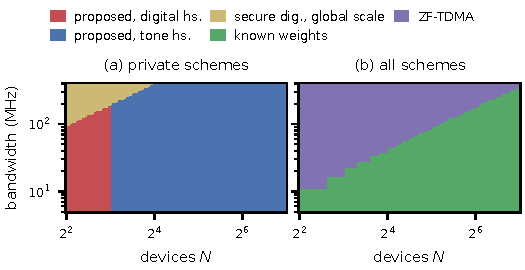
\includegraphics[width=\linewidth]{fig_regime.pdf}
\caption{Fastest scheme per token in the $(N,\text{bandwidth})$ plane, Qwen3-4B, $M=4$, $\tau=0.5$~ms, operating SNR 15~dB, with the required SNRs of the 8k sweep, $L=32$, $\nu=4$ and the measured ring sizes of Section~\ref{sec:exp}: (a) among schemes that reveal neither weights nor per-device data; (b) among all schemes.}
\label{fig:regime}
\end{figure}

\subsection{Robustness}

\emph{Common-mode errors.} A gain error common to all streams of all devices cancels in the analog ratio~\eqref{eq:estimator}; in the split ratios it scales the numerator only, so the FC must calibrate its own gain.

\emph{Device-specific errors.} Imperfect CSI or a residual phase at device $j$ multiplies its streams by a complex factor whose real part $\lambda_j$ attenuates them and whose imaginary part leaks each stream into its quadrature partner. Unlike saturation, the device does not know $\lambda_j$, so the arrived weight is $\lambda_ja_j$ while it reports $a_j$: by Proposition~\ref{prop:selfconsistency} the numerator shrinks by $\sum_j(1-\lambda_j)a_j\obar_j$. For a phase error of standard deviation $\sigma_\phi$ this is a common shrinkage of about $\sigma_\phi^2/2$, i.e., 1.5\% at $10^\circ$ and 6\% at $20^\circ$.

\emph{Frequency selectivity.} By Corollary~\ref{cor:coherence}, a payload that spans $C$ coherence blocks costs a non-saturating design $10\log_{10}C$~dB when the devices back off to their weakest block.

\emph{Heterogeneous path loss.} By Theorem~\ref{thm:bottleneck}, large-scale gains enter through $S=\sum_jd_j^2/\beta_j$: a device that holds mass behind a weak link dominates the bottleneck of a non-saturating design. The noise-matched report caps such a device automatically (Proposition~\ref{prop:kappa}) but attenuates its data. A digital fallback avoids this loss: the $k\ge2$ devices with the weakest effective gains, which the FC selects from the gains alone, securely aggregate their partials $(d_j,\vn_j)$ instead of transmitting over the air, and the FC adds their exact sum to its anchor. The cost is $kH(d_v+1)$ masked values per layer.

%==============================================================================
\section{Experiments}
\label{sec:exp}
%==============================================================================

All schemes share the model of Section~\ref{sec:model}: per-device peak power, real noise of unit variance per stream and $\snr=P$. ``Required SNR'' is the smallest SNR at which a metric reaches a target, interpolated linearly between grid points; ``--'' means that the target is not met on the grid. Unless stated otherwise, the ladder step is $\Delta=3$~dB, the tone handshake uses $\nu=4$ REs per level and $\alpha=10^{-3}$, and the digital handshake uses $q=256$ with its false zeros simulated. ``Proposed'' denotes Algorithm~\ref{alg:ladder} with both components and $\kappa=1$. Code and raw results are available at \url{https://github.com/zr0212-boom/aircomp-softmax}.

\subsection{Verification of the Analysis}

Every closed form was verified by Monte Carlo with $4\times10^5$--$10^6$ trials (69 checks), for uniform, geometric and attention-like weight profiles with and without heterogeneous path loss: the law~\eqref{eq:bottleneck} of $B$, its forms for $C=2,4$ coherence blocks and for the noise-matched report~\eqref{eq:kappa_law} with $\kappa\in\{0.3,1,3\}$, and the Nakagami law~\eqref{eq:bottleneck_m}, all within a CDF error of $2.2\times10^{-3}$; the distortion bound of Proposition~\ref{prop:kappa}(i), which is attained; the saturation law~\eqref{eq:psat} and its two other forms; both outage expressions of Theorem~\ref{thm:outage}; the bounds of Proposition~\ref{prop:combiner}; the false-alarm and miss probabilities of Proposition~\ref{prop:detection} within 4\% and 3\%; and Theorem~\ref{thm:converse}, where the ladder meets $W/(2K)$ on a uniform range and the optimum found by dynamic programming for Gaussian $X$ is within 4\% of the high-resolution value.

\subsection{Sharded-KV LLM Decoding}

\emph{Setup.} We use Qwen3-4B-Instruct and Qwen3-8B~\cite{qwen3} and Llama-3.1-8B-Instruct~\cite{llama3} in bfloat16; all have $H=32$ query heads with $d_v=128$. The FC holds the first 64 tokens and everything from the question on; the context in between is split into $N$ contiguous shards, and the attention of every query from the question on, in every layer and head, is merged over the air. In the fidelity task, the last 256 positions of a $T$-token text from WikiText-103~\cite{merity2017wikitext} are teacher-forced and compared with the exact shard merge, over 4 text segments and 4 channel draws, i.e., 16 samples per configuration. Channels are i.i.d.\ Rayleigh per layer and position and shared by the heads of a layer; $\sigma_o$, $V_{\max}$ and the ladder range are calibrated per layer and head on a disjoint text. The target is an NLL increase of 0.05~nats. The bfloat16 difference between the exact merge and the native attention kernel, a KL divergence of $5\times10^{-4}$--$10^{-3}$, bounds the resolution of any comparison. All schemes of a configuration see the same segments, channels and noise, so we report differences of required SNRs with paired bootstrap intervals (2000 resamples), which are tighter than those of the individual values (about $\pm1.5$~dB). The SNR grid is $-15$ to 25~dB in steps of 2.5~dB (from 0~dB for the designs that need more than that).

\emph{Baselines.} Three known-weight baselines reveal every $d_j$ to the FC: the genie scale~\eqref{eq:genie} with the exact denominator; the threshold scale of AirMoE~\cite{yang2026airmoe}, solved exactly per instance, with the exact denominator; and ``AirMoE-eff'', the same scale with the denominator of the arrived weights, i.e., AirMoE strengthened with our component~A. The private-weight references are the analog ladder and the non-saturating split ratio with its overflow fallback and consistency check, both with the tone handshake.

\emph{Choice of $\kappa$.} The rule was fixed before the test runs: on the CPython documentation as development corpus (Qwen3-4B, 8k, $N=8,32,64$), take the better of $\kappa=0.3$ and $\kappa=1$ by the mean required SNR on the 0--25~dB grid. The result was $\kappa=1$ (0.7 against 1.5~dB), which is used for every model, context length and $N$ on WikiText.

\begin{table*}[t]
\centering
\caption{SNR (dB) at which the NLL increase falls to 0.05~nats, $M=4$. Known-weight designs reveal every $d_j$ to the FC. Gaps: required SNR of the proposed design with the digital handshake minus that of the best known-weight design (AirMoE-eff; $^\dagger$AirMoE) and minus that of the non-saturating split ratio, with paired 95\% bootstrap intervals.}
\label{tab:llm}
\setlength{\tabcolsep}{3.5pt}
\begin{tabular}{@{}lcc ccc cccc cc@{}}
\toprule
 & & & \multicolumn{3}{c}{Known weights} & \multicolumn{4}{c}{Private weights} & \multicolumn{2}{c}{Gap of proposed (digital) to} \\
\cmidrule(lr){4-6}\cmidrule(lr){7-10}\cmidrule(l){11-12}
Model & Context & $N$ & Genie & AirMoE & AirMoE-eff & \shortstack{Analog\\ladder} & \shortstack{Non-sat.\\split} & \shortstack{Proposed\\(tone)} & \shortstack{Proposed\\(digital)} & best known weights & non-sat.\ split \\
\midrule
\tabinput{tables/tab_llm}
\bottomrule
\end{tabular}
\end{table*}

\emph{Fidelity.} Table~\ref{tab:llm} lists the required SNRs and Fig.~\ref{fig:llm} the curves of one configuration. Five observations hold for all models and context lengths. First, the proposed design with the digital handshake needs $-8.4$ to $8.4$~dB, which is 4.7--12.3~dB less than the non-saturating split ratio, with every interval excluding zero, and 9--16~dB less than the analog ladder. Second, it needs 1.8--9.1~dB less than known-weight aggregation at the genie scale and is on par with or better than AirMoE with the exact denominator ($-7.7$ to $+1.3$~dB): a private design that lets devices saturate in a controlled way outperforms a known-weight design that does not. Third, the strongest baseline, AirMoE-eff, remains 0.2--4.1~dB ahead (1.0--3.0~dB for Qwen3-4B, 0.2--2.6~dB for Llama-3.1-8B, 0.3--4.1~dB for Qwen3-8B); the interval includes zero in 3 of the 24 configurations. This is the price of private weights: a per-device budget cannot balance the total distortion against the noise as the centralized threshold does. Fourth, the tone handshake costs 0.7--11.7~dB relative to the digital one, most for Llama-3.1-8B, whose operating point is lowest: the proposed design then operates where tones are missed (for Qwen3-4B at 0~dB, the detected level is below the true one in 76--91\% of the instances), and although component~A keeps the misses harmless in the sense of Proposition~\ref{prop:eff}, the scale is no longer matched to the noise. The tone variant is still 0.2--5.1~dB better than the non-saturating split ratio with the same tones. Fifth, the required SNR does not grow with the number of devices: for Qwen3-4B at 8k it is 1.2, 2.8, 2.0, 1.5, 0.7 and $-0.1$~dB for $N=4$ to 128, whereas time-division ZF, which meets the target at about 0~dB, needs $\lceil2N/M\rceil$ slots. Longer contexts cost more: from 8k to 32k at $N=32$, the proposed design loses 5--8~dB and AirMoE-eff 4--10~dB. With $M=8$ antennas (Qwen3-4B, 8k), it needs 1.2, $-0.1$ and $-0.1$~dB for $N=8$, 32 and 64, i.e., 0.8--1.6~dB less than with four, at gaps of 1.0--2.8~dB to AirMoE-eff.

The attention statistics explain the size of these gains. With unit gains, $\log_{10}S$ spans 2.0--2.3 decades between the 10th and 90th percentiles of the decode positions in the median head and 3.1--3.7 decades in the 90th-percentile head, and the participation ratio is small (median $\Neff$ of 2.0--3.1, 4.5--8.3 and 6.4--13.8 for $N=8$, 32 and 64 at 8k): a few shards hold the mass, and the bottleneck is typically set by a device whose contribution to the output is minor. At the operating point of the proposed design nearly every instance has a saturated device (96--100\% at 0--5~dB for Qwen3-4B), yet the saturated mass $\sum_j(d_j-a_j)$ is only 5--10\% of the denominator.

\begin{figure}[t]
\centering
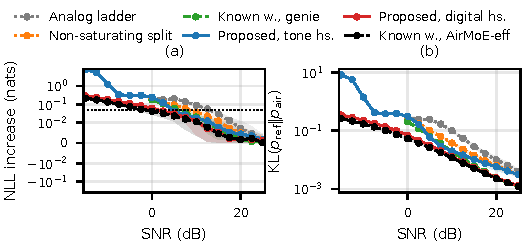
\includegraphics[width=\linewidth]{fig_llm_curves.pdf}
\caption{Qwen3-4B, 8k context, $N=32$ devices, $M=4$: (a) NLL increase and (b) KL divergence versus SNR (4 segments $\times$ 4 channel draws; shaded: 95\% confidence interval).}
\label{fig:llm}
\end{figure}

\emph{Design study.} Table~\ref{tab:design} separates the components for Qwen3-4B at 8k. Component~A alone changes little ($-1.0$ to $0.0$~dB against the non-saturating split ratio), as expected: it makes saturation harmless but does not create any. Component~B creates it: with both components the required SNR falls by 3.9--7.0~dB with the digital handshake and by 1.4--3.8~dB with tones. With the digital handshake, B with the exact denominator is as good as A+B (differences of $-0.1$ to $+0.3$~dB, intervals within $\pm1.3$~dB), in line with Proposition~\ref{prop:kappa}(i); with tones, B needs A: the analog denominator is 1.3--3.7~dB worse. The noise-matched rule is also as good as or better than a fixed 3~dB offset of the scale (by 0.1--1.1~dB). In $\kappa$ the design is monotone over the tested range: $\kappa=3$ is a further 0.6--1.1~dB better than the pre-registered $\kappa=1$ on this configuration, so the reported numbers are not tuned to the test set and leave some margin. A step of 6~dB costs 0.8--1.2~dB and a step of 1.5~dB gains 0.4~dB, consistent with the mean quantization penalty $\Delta/2$ of Theorem~\ref{thm:converse}, so the ladder can be halved at about 1~dB. For the tones, $\nu=8$ instead of 4 gains 1.1--1.3~dB and $\nu=2$ loses 1.4--1.9~dB. Component~A is worth 1.0--3.1~dB to the AirMoE baseline as well.

\begin{table}[t]
\centering
\caption{Design study, Qwen3-4B, 8k, $M=4$: required SNR (dB). A: saturation-aware denominator; B: noise-matched report.}
\label{tab:design}
\setlength{\tabcolsep}{2.5pt}
\begin{tabular}{@{}lccc@{}}
\toprule
Design & $N=8$ & $N=32$ & $N=64$ \\
\midrule
\tabinput{tables/tab_design}
\bottomrule
\end{tabular}
\end{table}

\emph{One-round designs.} Can the handshake round be saved? Not with the designs we know. The best blind scale, a fixed quantile of $B$ chosen on the test set, needs 27.5--28.4~dB for Qwen3-4B (19.3--19.5~dB for Llama-3.1-8B, 28.2--28.5~dB for Qwen3-8B); the 0.5 quantile never reaches the target and the 0.99 quantile fails or needs 31--47~dB, which is the dilemma of Corollary~\ref{cor:blind}. Component~A lowers the best blind scale to 22.5--23.3~dB, and a stale ladder that reuses the level of the previous position needs 23.2--28.3~dB with A, with or without B. The handshake is thus worth more than 20~dB.

\emph{Channel impairments.} Table~\ref{tab:real} repeats the $N=32$ configuration under impairments; phase and CSI errors use the I/Q model of Section~\ref{sec:regime}, including the leakage between quadrature streams. Independent channels per head and channels that stay constant over the session cost nothing. Spanning $C=2$ and 4 coherence blocks costs the proposed design 2.2 and 4.7~dB and the known-weight designs 2.0--2.8 and 3.8--5.4~dB, against the 3 and 6~dB of Corollary~\ref{cor:coherence} for a non-saturating scale. Phase errors of up to $10^\circ$, ramps of up to $45^\circ$ across the payload and a CSI error of 0.05 cost the proposed design at most 0.6~dB; $20^\circ$ and an NMSE of 0.1 cost 1.5 and 2.4~dB, whereas the non-saturating split ratio loses 4.2 and 9.6~dB. A large-scale spread of 4 and 8~dB costs 2.2 and 9.3~dB, of which the digital fallback of the two weakest devices recovers 2.5 and 2.7~dB; the known-weight baselines lose as much (2.7 and 9.6~dB for AirMoE-eff), so the spread is a property of the task rather than of private weights. With all impairments combined, the proposed design needs 4.2~dB for Qwen3-4B and $-0.9$~dB for Llama-3.1-8B. Across all rows the gap to AirMoE-eff stays between 1.4 and 3.0~dB.

\begin{table}[t]
\centering
\caption{Channel impairments, Qwen3-4B, 8k, $N=32$, $M=4$: required SNR (dB). Spread: log-normal large-scale gains. Combined: per-head channels, $C=2$, phase error $10^\circ$, ramp $20^\circ$, CSI NMSE 0.01 and 4~dB spread; fallback: 4 / 8~dB spread.}
\label{tab:real}
\setlength{\tabcolsep}{2.5pt}
\begin{tabular}{@{}lccccc@{}}
\toprule
 & \multicolumn{2}{c}{Known weights} & \multicolumn{3}{c}{Private weights} \\
\cmidrule(lr){2-3}\cmidrule(l){4-6}
Scenario & Genie & \shortstack{AirMoE\\-eff} & \shortstack{Non-sat.\\split} & \shortstack{Prop.\\(tone)} & \shortstack{Prop.\\(dig.)} \\
\midrule
\tabinput{tables/tab_real}
\bottomrule
\end{tabular}
\end{table}

\emph{Retrieval.} In the needle-in-a-haystack task, one or four passphrases are placed at depths of 10\%, 50\% and 90\% of a WikiText haystack, with 60 prompts and 2 channel draws (120 trials). A trial succeeds if every token of the exact-merge answer is the arg-max under the over-the-air merge, which is equivalent to greedy decoding with the same channel draws (against greedy generation the difference is $+0.5\pm0.4$ percentage points over 8 configurations). Table~\ref{tab:niah} reports the accuracy. With the digital handshake the proposed design is within one trial of the ceiling from 10~dB on in all 16 configurations (Table~\ref{tab:niah} lists those with $N\ge32$) and loses at most 1.7 points with one key and 3.3 points with four keys at 5~dB; in no cell is it below AirMoE-eff. With tones it needs 10~dB to come within two trials of the ceiling and fails at 5~dB with four keys.

\begin{table}[t]
\centering
\caption{NIAH accuracy (\%), teacher-forced, 120 trials, $M=4$. Ceiling: teacher-forced accuracy without the channel.}
\label{tab:niah}
\setlength{\tabcolsep}{1.7pt}
\begin{tabular}{@{}lcccccccc@{}}
\toprule
 & & \multicolumn{2}{c}{AirMoE-eff} & \multicolumn{2}{c}{Prop.\ (dig.)} & \multicolumn{3}{c}{Prop.\ (tone)} \\
\cmidrule(lr){3-4}\cmidrule(lr){5-6}\cmidrule(l){7-9}
Model, context, $N$ & Ceil. & 5 & 10 & 5 & 10 & 5 & 10 & 15~dB \\
\midrule
\tabinput{tables/tab_niah}
\bottomrule
\end{tabular}
\end{table}

\subsection{Secure Digital Merge and Latency}

\emph{Ring size at matched accuracy.} We implemented the secure digital merge in fixed point, on an error-free link, and searched the ring size $b$ at which the NLL increase stays below 0.05~nats for every $N$. With an offline scale per head (the calibrated maximum with an 8-bit margin for queries outside the calibration range), it needs 32~bits for Qwen3-4B at 8k, 36~bits at 32k and 28~bits for the two 8B models. With an oracle scale per instance, a lower bound for any public scale, 10--12~bits suffice. A plain bfloat16 merge also meets the target.

\emph{Latency.} Table~\ref{tab:latency} evaluates Section~\ref{sec:regime} for Qwen3-4B (36 layers) at an operating SNR of 15~dB with the required SNRs of the 8k sweep, $\tau=0.5$~ms, an RE efficiency of 0.72, a digital rate of Shannon capacity minus 3~dB with $\min(M,N)$-fold multiplexing, which favors the digital schemes, $L=32$, $b_A=\FXBITS$ and $b_w=16$~bits. The secure digital merge is given its measured ring sizes; for the per-instance scale we charge the second round trip but not the handshake payload. At 20~MHz the proposed design, in the faster of its two forms, is 1.4--14.5 times faster than the per-instance secure merge for $N=4$ to 128 and 2.4--42 times faster than the offline-scale one; at 100~MHz the factors are 1.1--5.4 and 0.95--14, the only exception being $N=4$, where the offline-scale merge is 5\% faster. The digital handshake is the faster form up to $N=8$; beyond that its $NHL$ bytes dominate and the tone handshake, whose cost does not depend on $N$, is preferable. Schemes that reveal the weights or the per-device data remain faster: known-weight aggregation by 1--18~ms, and time-division ZF for $N\le8$ at 20~MHz and $N\le32$ at 100~MHz (Fig.~\ref{fig:regime}).

\begin{table}[t]
\centering
\caption{Per-token latency (ms) at matched accuracy, Qwen3-4B, $M=4$, SNR 15~dB. Private schemes reveal neither weights nor per-device data. Secure digital merge: 12-bit ring with a per-instance scale (lower bound) and 36-bit ring with an offline scale.}
\label{tab:latency}
\setlength{\tabcolsep}{2.5pt}
\begin{tabular}{@{}lccccccc@{}}
\toprule
 & \multicolumn{4}{c}{Private} & \multicolumn{3}{c}{Not private} \\
\cmidrule(lr){2-5}\cmidrule(l){6-8}
 & \multicolumn{2}{c}{Proposed} & \multicolumn{2}{c}{Secure dig.} & Known & ZF- & Dig. \\
Band, $N$ & dig. & tone & inst. & offl. & w. & TDMA & bf16 \\
\midrule
\tabinput{tables/tab_latency}
\bottomrule
\end{tabular}
\end{table}

\subsection{Spatial-Field Estimation}

\emph{Setup.} As in~\cite{sato2026awa}, a log-normal shadowing field (8~dB, Gudmundson correlation distance 100~m~\cite{gudmundson1991correlation}) covers $500\times500$~m$^2$ and measurements carry 1~dB noise; each round estimates the field at 10 query points that share one channel draw, and we report the median per-round RMSE over 2000 rounds. In product-of-experts (PoE) regression, 256 measurements are partitioned among $K$ devices by a grid, with the local posterior precisions as weights; in Nadaraya--Watson (NW) regression, each of $K$ sensors holds one measurement (bandwidth 30~m) and the FC adds a prior pseudo-observation. Adaptively weighted averaging (AWA)~\cite{sato2026awa} clips the weights to bounds tuned per SNR on a calibration set, an optimistic stand-in for its Bayesian optimization. ``Ladder-T'' is the analog ladder with weak-link truncation~\cite{zhu2020broadband}: devices whose gain is below a tuned quantile are not scheduled. The proposed design uses the same $\kappa=1$ and $\Delta=3$~dB as for the LLMs, without any tuning, and 16 tone observations per level.

\emph{Results.} Table~\ref{tab:field} summarizes the single-antenna results. With equal path loss the proposed design is within 0.13~dB of AirMoE-eff at 10~dB with either handshake and outperforms AWA by 0.4--1.6~dB. With a 10~dB log-normal spread of the large-scale gains (unit mean), non-saturating designs collapse, since a few devices with weak links dominate $S=\sum_jd_j^2/\beta_j$: the genie scale with known weights is at 8.7--15.9~dB at 10~dB. The noise-matched report caps these devices by itself: the proposed design stays within 0.02--1.7~dB of AirMoE-eff (digital handshake; at most 0.7~dB with tones) and outperforms AWA by 3.5--16~dB at 10~dB. Without any tuning it is within 0.1~dB of the tuned truncation or better in all entries but one (PoE with $K=4$ at 10~dB). With few devices and a large spread, tones do better than the digital handshake at 10--20~dB because the tones of the weakest devices go undetected, an implicit truncation; at 0~dB the same effect makes the tone variant fail for PoE with $K=4$.

\begin{table*}[t]
\centering
\caption{Spatial-field estimation: median RMSE (dB) at 10 / 20~dB, $M=1$. Spread: unit-mean log-normal large-scale gains with 10~dB standard deviation. AirMoE-eff knows every weight; Ladder-T and AWA are tuned per SNR.}
\label{tab:field}
\setlength{\tabcolsep}{5pt}
\begin{tabular}{@{}llccccccc@{}}
\toprule
Path loss & Task, $K$ & Ideal & AirMoE-eff & Proposed (digital) & Proposed (tone) & Non-sat.\ split & Ladder-T & AWA~\cite{sato2026awa} \\
\midrule
\tabinput{tables/tab_field}
\bottomrule
\end{tabular}
\end{table*}

%==============================================================================
\section{Conclusion}
\label{sec:conclusion}
%==============================================================================

When the weights of a normalized aggregation are private, over-the-air computation is limited by the mass-weighted weakest link, whose distribution is an exact Fr\'echet law with scale $\sum_jd_j^2/\beta_j$. On attention weights, the best weight-blind scale therefore needs 19--28~dB. An anonymous ladder handshake is the best that a scale which never saturates can do with a given number of revealed bits, and it loses half a ladder step. The larger loss is the refusal to saturate itself. Two components remove it without revealing any weight: a securely aggregated denominator of the weights that actually arrive, which keeps the ratio a convex combination under any saturation, and a noise-matched level report, which bounds every device's distortion by $\kappa$ noise variances and turns the Fr\'echet bottleneck into a bounded one. In sharded-KV decoding of three LLMs with up to 128 devices and 32k-token contexts, the resulting design is near-lossless at $-8$ to $8$~dB, 5--12~dB below the non-saturating split ratio and 2--9~dB below known-weight aggregation at the genie scale, with a required SNR that does not grow with the number of devices. Against the strongest known-weight baseline, the threshold scale of AirMoE with the same denominator, it loses 0.2--4.1~dB; this is the measured price of private weights. The handshake is the main cost. In its digital form it is reliable at any SNR but grows with the number of devices; tones are cheap but cost 1--12~dB at the low SNRs at which the design otherwise operates; and one-round designs without it need more than 20~dB more. Among schemes that reveal neither weights nor per-device data, the design is up to 14 times faster than a secure digital merge at the ring size that the same accuracy requires, except for few devices in wide bands, whereas schemes that reveal the weights or the data remain faster. Open problems are a decentralized report that balances the total distortion as the centralized threshold does, a handshake whose cost grows with neither the number of devices nor the inverse SNR, and combiners matched to private weights.


\appendices
%==============================================================================
\section{Proofs}
\label{app:proofs}
%==============================================================================

\subsection{Theorem~\ref{thm:bottleneck} and Corollaries~\ref{cor:tail} and~\ref{cor:coherence}}
By independence, $\Prob\{B\le x\}=\prod_j\Prob\{|\tilde h_j|^2\ge d_j^2/(\beta_jx)\}$, and $\Prob\{|\tilde h_j|^2\ge u\}=Q(m,mu)$ for $|\tilde h_j|^2\sim\mathrm{Gamma}(m,1/m)$, which gives~\eqref{eq:bottleneck_m}; for $m=1$, $Q(1,u)=e^{-u}$ and the product is $e^{-S/x}$. For Corollary~\ref{cor:coherence}, $\min_cg_{jc}$ is exponential with mean $\beta_j/C$. For Corollary~\ref{cor:tail}, $e^{-S/x}=1/2$ gives the median, $1-e^{-S/x}=S/x+O(x^{-2})$ gives the tail and $\E[B]=\int_0^\infty\Prob\{B>x\}\,dx=\infty$, and $S/B\sim\mathrm{Exp}(1)$ gives~\eqref{eq:effective_snr}. Under Nakagami-$m$ fading, with $u_j=md_j^2/(\beta_jx)\to0$, $1-Q(m,u)=u^m/\Gamma(m+1)\,(1+O(u))$, hence $\Prob\{B>x\}=\sum_ju_j^m/\Gamma(m+1)\,(1+o(1))$, which is~\eqref{eq:tail_m}; the tail is regularly varying with index $-m$. \hfill$\blacksquare$

\subsection{Theorem~\ref{thm:outage}}
Under genie scaling, $\hat D-d_A-D=z_0/\eta_{\rm g}$ with $1/\eta_{\rm g}^2=B/P$, and $1/B=Y/S$ with $Y\sim\mathrm{Exp}(1)$ independent of $z_0$. Hence $p_{\rm out}=\Prob\{Y<az_0^2\}=1-\E[e^{-az_0^2}]$ with $a=S/(\epsilon PD^2)$, and $\E[e^{-az_0^2}]=(1+2a)^{-1/2}$ for $z_0\sim\mathcal{N}(0,1)$; $a=1/(\epsilon\,\snr\,\Neff)$ for unit gains. For complex noise $w$ of unit variance, $|w|^2\sim\mathrm{Exp}(1)$ and $1-\E[e^{-a|w|^2}]=a/(1+a)$. \hfill$\blacksquare$

\subsection{Proposition~\ref{prop:moments}}
(i) Given everything but $z_0$, $\hat D$ is Gaussian, so its density is bounded away from zero near the origin and $\E[1/|\hat D|]=\infty$, while $\hat\vn$ is independent of $z_0$ and nonzero with positive probability.
(ii) Write $\hat\vn=\vn+\sigma_o\vz/\eta$ with $\|\vn\|\le(d_A+D)V_{\max}$, where $\vz$, $z_0$ and $\eta$ are independent. Sufficiency: $\|\hat\vo\|\le\|\hat\vn\|/d_A$, so $\E\|\hat\vo\|^k<\infty$ whenever $\E[\eta^{-k}]=P^{-k/2}\E[B^{k/2}]<\infty$. Necessity: on $\{z_0\le0\}$ the denominator is at most $d_A+D$, and on $\{\|\vz\|\ge1\}\cap\{1/\eta\ge c\}$ with $c=2(d_A+D)V_{\max}/\sigma_o$ we have $\|\hat\vn\|\ge\sigma_o\|\vz\|/(2\eta)$; by independence, $\E\|\hat\vo\|^k$ is at least a positive constant times $\E[\eta^{-k}\mathbb{1}\{\eta^{-1}\ge c\}]$, which is infinite whenever $\E[B^{k/2}]=\infty$. Corollary~\ref{cor:tail} gives $k<2m$.
(iii) The denominator in~\eqref{eq:estimator} is at least $\|\hat\vn\|/V_{\max}$. \hfill$\blacksquare$

\subsection{Theorem~\ref{thm:saturation} and Corollary~\ref{cor:blind}}
Device $j$ saturates if and only if $g_j<\tau d_j^2$, so no device saturates with probability $\prod_je^{-\tau d_j^2/\beta_j}=e^{-\tau S}$; averaging over $S$ and inserting $\tau=\ln\frac{1}{1-\delta}/\hat S$ give the other two forms. For the corollary, the noise ratio is $(S/B)/(\tau_\delta S)$ and $S/B\sim\mathrm{Exp}(1)$ has median $\ln2$. (i) Since $(1-e^{-\tau S})/\tau\uparrow S$ as $\tau\downarrow0$, monotone convergence gives $1-\mathcal{L}_S(\tau)=\tau\E[S](1+o(1))$. (ii) Integration by parts gives $1-\mathcal{L}_S(\tau)=\tau\int_0^\infty e^{-\tau s}\Prob\{S>s\}\,\mathrm{d}s$, and Karamata's Tauberian theorem~\cite[Thm.~1.7.1]{bingham1987regular} yields $1-\mathcal{L}_S(\tau)\sim\Gamma(1-\alpha)\tau^\alpha\varsigma(1/\tau)$; the inverse of a regularly varying function of index $\alpha$ has index $1/\alpha$~\cite[Thm.~1.5.12]{bingham1987regular}. \hfill$\blacksquare$

\subsection{Propositions~\ref{prop:ladder}--\ref{prop:leakage}}
\emph{Ladder gap.} For $\kappa=0$ and $\ell_{\min}\Delta\le10\log_{10}B\le\ell_{\max}\Delta$, $\ell^\star=\lceil10\log_{10}B/\Delta\rceil$, so $B\le10^{\ell^\star\Delta/10}<10^{\Delta/10}B$ and $\eta^2=P10^{-\ell^\star\Delta/10}\le\eta_{\rm g}^2$; below $\ell_{\min}$ the scale is smaller still.

\emph{Tone detection.} Given the levels, the sample of level $\ell$ on RE $k$ and antenna $m$ is $\sum_{j:\ell_j=\ell}\sqrt{P}h_{jkm}+w_{km}$, circularly symmetric Gaussian with variance $PS_\ell+2$, independently over the $M\nu$ pairs $(k,m)$, so $E_\ell$ is Gamma distributed with shape $M\nu$ and scale $PS_\ell+2$. Every level above $\ell^\star$ is empty and exceeds $\theta$ with probability $Q(M\nu,\theta/2)=\alpha/L$; a union bound gives the first claim. A miss requires $E_{\ell^\star}\le\theta$, and $P(a,x)\le x^a/\Gamma(a+1)$.

\emph{Leakage.} (i) The sum of level $\ell$ is $Y_\ell=\sum_{j:\ell_j\ge\ell}\rho_{j\ell}$, which is zero if the sum is empty and otherwise uniform on $\mathbb{Z}_q$, because a sum of independent elements of a finite group of which at least one is uniform is uniform. Given the levels, the $Y_\ell$ are independent, and the law of each depends only on $\mathbb{1}\{\ell\le\ell^\star\}$. Hence $\mathbf{d}\to\ell^\star\to Y$ is a Markov chain given $\mathbf{g}$, and $I(\mathbf{d};Y\mid\mathbf{g})\le H(\ell^\star\mid\mathbf{g})\le\log_2(L+1)$. (ii) Given the levels, the samples of level $\ell$ are independent Gaussian with variance $Pn_\ell\beta+2$, $n_\ell=|\{j:\ell_j=\ell\}|$, since the FC does not know the per-device channels. Hence $I(\mathbf{d};Y\mid\mathbf{g})\le H((n_\ell)_\ell)$, at most the logarithm of the number of histograms of $N$ devices over $L+1$ levels. \hfill$\blacksquare$

\subsection{Theorem~\ref{thm:converse} and Corollary~\ref{cor:tradeoff}}
Given the message $k$, non-saturation requires $10\log_{10}(P/\eta_k^2)\ge X$ for every $X$ mapped to $k$, so the best scale for message $k$ is the supremum of its cell $\mathcal{C}_k$ and the penalty is $\sup\mathcal{C}_k-X$. Replacing each cell by the interval between its infimum and supremum, and assigning the overlap of two intervals to the one with the smaller supremum, does not increase any penalty, so interval partitions suffice. A randomized design is a mixture of deterministic ones, and the mean penalty is linear in the mixture. (i) For uniform $X$, a cell of length $l_k$ contributes $l_k^2/(2W)$, and $\sum_kl_k^2\ge W^2/K$ by the Cauchy--Schwarz inequality, with equality for equal lengths. (ii) At high resolution, a cell of length $l_k$ around $x_k$ contributes $f(x_k)l_k^2/2$; minimizing $\sum_kf(x_k)l_k^2/2$ subject to $\sum_kl_k=W$ gives $l_k\propto f(x_k)^{-1/2}$ and the stated value, and $(\int\sqrt f)^2\le W\int f=W$. For the corollary, a message of $k$ bits takes at most $K=2^k$ values. \hfill$\blacksquare$

\subsection{Lemma~\ref{lem:projection} and Propositions~\ref{prop:selfconsistency}--\ref{prop:kappa}}
The weights $d_A/(d_A+D)$ and $d_j/(d_A+D)$ of~\eqref{eq:target} are nonnegative and sum to one on vectors of norm at most $V_{\max}$, hence $\|\vn_A+\sum_jd_j\obar_j\|\le(d_A+D)V_{\max}$; the same holds with $\lambda_jd_j$ or $a_j$ in place of $d_j$, which proves the convexity claims, and the bias of the split ratio follows by subtracting $\vo$. For~\eqref{eq:eff_bias}, write $(d_A+D)(\vo-\tilde\vo)=\vn_A+\sum_jd_j\obar_j-(d_A+A)\tilde\vo-(D-A)\tilde\vo$ and use $(d_A+A)\tilde\vo=\vn_A+\sum_ja_j\obar_j$ and $D-A=\sum_j(d_j-a_j)$. Proposition~\ref{prop:kappa}: (i) if device $j$ saturates, $a_j=c_ju\ge c_jr_j$, so $0<d_j-a_j\le d_j-c_jr_j=\sqrt\kappa\,r_j\le\sqrt\kappa\,u$. (ii) $r_j\le d_j/c_j$ and $r_j\le d_j/\sqrt\kappa$. (iii) $\tilde B\le x$ if and only if $\sqrt{g_j}\ge d_j/\sqrt x-\sqrt{\kappa/P}$ for every $j$; the events are independent and $\Prob\{g_j\ge t^2\}=e^{-t^2/\beta_j}$ for $t\ge0$. \hfill$\blacksquare$

\subsection{Proposition~\ref{prop:combiner}}
By the Cauchy--Schwarz inequality, $|\vm^{\mathsf H}\vh_j|^2\le\|\vh_j\|^2$, so $B_{\vm}\ge\max_jd_j^2/\|\vh_j\|^2$, and the norms $\|\vh_j\|^2$ are independent and Gamma distributed with shape $M$ and scale $\beta_j$, which gives~\eqref{eq:comb_upper}. For the max--min combiner, fix any unit vector $\vm_0$ independent of the channels. Then $B_{\vm}\le d_{\max}^2/\min_j|\vm^{\mathsf H}\vh_j|^2\le d_{\max}^2/\min_j|\vm_0^{\mathsf H}\vh_j|^2$, and the gains $|\vm_0^{\mathsf H}\vh_j|^2$ are independent and exponential with means $\beta_j$, so their minimum is exponential with rate $\sum_j1/\beta_j$, which gives~\eqref{eq:comb_lower}. \hfill$\blacksquare$


%==============================================================================
% References (inline bibliography; IEEE style).
%==============================================================================
\begin{thebibliography}{99}

\bibitem{lin2024infinite} B.~Lin \emph{et al.}, ``Infinite-LLM: Efficient LLM service for long context with DistAttention and distributed KVCache,'' \emph{arXiv:2401.02669}, 2024.

\bibitem{acharya2025star} S.~Acharya, F.~Jia, and B.~Ginsburg, ``Star Attention: Efficient LLM inference over long sequences,'' in \emph{Proc. Int. Conf. Mach. Learn. (ICML)}, 2025.

\bibitem{bhatia2025helix} N.~Bhatia \emph{et al.}, ``Helix parallelism: Rethinking sharding strategies for interactive multi-million-token LLM decoding,'' \emph{arXiv:2507.07120}, 2025.

\bibitem{shyam2024tree} V.~Shyam \emph{et al.}, ``Tree attention: Topology-aware decoding for long-context attention on GPU clusters,'' \emph{arXiv:2408.04093}, 2024.

\bibitem{meta2025cp} A.~Yang \emph{et al.}, ``Context parallelism for scalable million-token inference,'' in \emph{Proc. Conf. Mach. Learn. Syst. (MLSys)}, 2025.

\bibitem{sato2022gpr} K.~Sato, ``Over-the-air Gaussian process regression based on product of experts,'' in \emph{Proc. IEEE GLOBECOM Workshops}, 2022, pp.~1814--1820.

\bibitem{sato2026awa} K.~Sato and K.~Ishibashi, ``Adaptively weighted averaging over-the-air computation and its application to distributed Gaussian process regression,'' \emph{IEEE Trans. Cogn. Commun. Netw.}, vol.~12, pp.~480--496, 2026.

\bibitem{nazer2007computation} B.~Nazer and M.~Gastpar, ``Computation over multiple-access channels,'' \emph{IEEE Trans. Inf. Theory}, vol.~53, no.~10, pp.~3498--3516, Oct. 2007.

\bibitem{goldenbaum2015nomographic} M.~Goldenbaum, H.~Boche, and S.~Sta\'nczak, ``Nomographic functions: Efficient computation in clustered Gaussian sensor networks,'' \emph{IEEE Trans. Wireless Commun.}, vol.~14, no.~4, pp.~2093--2105, Apr. 2015.

\bibitem{sahin2023survey} A.~\c{S}ahin and R.~Yang, ``A survey on over-the-air computation,'' \emph{IEEE Commun. Surveys Tuts.}, vol.~25, no.~3, pp.~1877--1908, 2023.

\bibitem{cao2020power} X.~Cao, G.~Zhu, J.~Xu, and K.~Huang, ``Optimized power control for over-the-air computation in fading channels,'' \emph{IEEE Trans. Wireless Commun.}, vol.~19, no.~11, pp.~7498--7513, Nov. 2020.

\bibitem{liu2020scaling} W.~Liu, X.~Zang, Y.~Li, and B.~Vucetic, ``Over-the-air computation systems: Optimization, analysis and scaling laws,'' \emph{IEEE Trans. Wireless Commun.}, vol.~19, no.~8, pp.~5488--5502, Aug. 2020.

\bibitem{yang2026airmoe} H.~Yang, Z.~Wang, and K.~Huang, ``AirMoE: Realizing over-the-air distributed mixture-of-experts inference at the wireless edge,'' \emph{arXiv:2608.22932}, 2026.

\bibitem{zhang2026logit} L.~Zhang, Y.~Jia, L.~Cao, D.~Wang, J.~Ren, and S.~Cui, ``Logit-aware MIMO AirComp for distributed mixture-of-experts LLM inference over wireless edge networks,'' \emph{arXiv:2610.03741}, 2026.

\bibitem{chen2024view} X.~Chen, K.~B.~Letaief, and K.~Huang, ``On the view-and-channel aggregation gain in integrated sensing and edge AI,'' \emph{IEEE J. Sel. Areas Commun.}, vol.~42, no.~9, pp.~2292--2305, Sep. 2024.

\bibitem{zhu2019mimo} G.~Zhu and K.~Huang, ``MIMO over-the-air computation for high-mobility multimodal sensing,'' \emph{IEEE Internet Things J.}, vol.~6, no.~4, pp.~6089--6103, Aug. 2019.

\bibitem{zhu2020broadband} G.~Zhu, Y.~Wang, and K.~Huang, ``Broadband analog aggregation for low-latency federated edge learning,'' \emph{IEEE Trans. Wireless Commun.}, vol.~19, no.~1, pp.~491--506, Jan. 2020.

\bibitem{evgenidis2024imperfect} N.~Evgenidis, V.~Papanikolaou, P.~D.~Diamantoulakis, and G.~K.~Karagiannidis, ``Over-the-air computing with imperfect CSI: Design and performance optimization,'' \emph{IEEE Trans. Wireless Commun.}, vol.~23, no.~6, pp.~6093--6108, Jun. 2024.

\bibitem{zhang2025jstsp} K.~Zhang, H.~He, S.~Song, J.~Zhang, and K.~B.~Letaief, ``Communication-efficient distributed on-device LLM inference over wireless networks,'' \emph{IEEE J. Sel. Topics Signal Process.}, vol.~19, no.~7, pp.~1301--1317, Oct. 2025.

\bibitem{bonawitz2017secagg} K.~Bonawitz \emph{et al.}, ``Practical secure aggregation for privacy-preserving machine learning,'' in \emph{Proc. ACM Conf. Comput. Commun. Secur. (CCS)}, 2017, pp.~1175--1191.

\bibitem{xiao2024streaming} G.~Xiao, Y.~Tian, B.~Chen, S.~Han, and M.~Lewis, ``Efficient streaming language models with attention sinks,'' in \emph{Proc. Int. Conf. Learn. Represent. (ICLR)}, 2024.

\bibitem{bingham1987regular} N.~H.~Bingham, C.~M.~Goldie, and J.~L.~Teugels, \emph{Regular Variation}. Cambridge, U.K.: Cambridge Univ. Press, 1987.

\bibitem{gudmundson1991correlation} M.~Gudmundson, ``Correlation model for shadow fading in mobile radio systems,'' \emph{Electron. Lett.}, vol.~27, no.~23, pp.~2145--2146, Nov. 1991.

\bibitem{llama3} A.~Grattafiori \emph{et al.}, ``The Llama 3 herd of models,'' \emph{arXiv:2407.21783}, 2024.

\bibitem{qwen3} Qwen Team, ``Qwen3 technical report,'' \emph{arXiv:2505.09388}, 2025.

\bibitem{merity2017wikitext} S.~Merity, C.~Xiong, J.~Bradbury, and R.~Socher, ``Pointer sentinel mixture models,'' in \emph{Proc. Int. Conf. Learn. Represent. (ICLR)}, 2017.

\end{thebibliography}


\end{document}
